%File: formatting-instruction.tex
\documentclass[letterpaper]{article}

\usepackage{aaai}
\usepackage{times}
\usepackage{helvet}
\usepackage{courier}
\usepackage{graphicx}
\usepackage{url}

\graphicspath{ {./images/} }

\frenchspacing
\setlength{\pdfpagewidth}{8.5in}
\setlength{\pdfpageheight}{11in}
\pdfinfo{
/Title (Multi-Agent System in Data Center environment)
/Author (Douglas Trajano)}
\setcounter{secnumdepth}{2}  
 \begin{document}
% The file aaai.sty is the style file for AAAI Press 
% proceedings, working notes, and technical reports.
%
\title{Multi-Agent System in Data Center environment}
\author{Douglas Trajano\\
Pontifical Catholic University of Rio Grande do Sul - PUCRS\\
School of Technology. Porto Alegre, Brazil\\
douglas.trajano@edu.pucrs.br\\
}
\maketitle
\begin{abstract}
\begin{quote}
In this paper, we introduce a multi-agent system in a data center environment. The system is composed of different types of agents, each of which has its own artifact, and the system is designed to solve all issues in the data center environment. The agents walk around the data center searching for issues, when they find an issue, they will try to solve it. The system is designed to solve all issues in the data center environment.
\end{quote}
\end{abstract}

\section{Introduction}

Nowadays, IT operations are crucial for business continuity. Information systems are used by companies in different processes and products, all these services are implemented in data centers. Critical incidents in data centers may impact the usability of these services and it needs to be handled in timely fashion by the engineering team to avoid financial losses or affect their end-users.

A data center is a building composed of computer systems, storage systems, infrastructure for power supply, telecommunications, environmental controls (e.g., air conditioning, fire suppression), and many other associated components. The complexity of these resources lies in the fact that all these components need to work together, if one of these components has an issue, it can affect other components. Engineers need to solve these issues in a timely fashion.

In this work, we introduce a multi-agent system in a data center environment. The environment simulates a data center plant with several racks, each rack has several servers. When a server is facing an issue, it will be marked as "red", and the agents will try to solve the issue. The system is designed to solve all issues in the data center environment.

This work is organized as follows. Section \ref{sec:relatedwork} is about the related work and the background of the problem. Section \ref{sec:approach} explains our approach to solve the problem. Section \ref{sec:experiments} describes our experiments and the results. Finally, we conclude with discussion and future directions in Section \ref{sec:conclusions}.

\section{Related work and background}\label{sec:relatedwork}

Modern software applications have to deal with an increasing level of autonomy of interconnected software systems. Multi-agent systems are a paradigm for modeling and engineering complex systems. \cite{boissier2020multi}

As the name says, Multi-Agent Systems (MAS) are systems made up of multiple agents. It has the capacity to build and understand a wide range of artificial social systems and can be applied in several different areas.\cite{wooldridge2009introduction}

JaCaMo \cite{boissier2013multi} is a multi-agent systems development platform that enables integration of three multi-agent programming dimensions: agents, organisations, and environment. A JaCaMo system, as shown in Figure 2.1, consists of the following platforms: Jason \cite{bordini2007programming} for agent development, CArtAgO \cite{bordini2009multi} for environment programming, and Moise \cite{hubner2007developing} for programming organisations. Therefore, JaCaMo integrates these three platforms for a uniform and consistent programming model, with the goal of simplifying the combination of these dimensions when programming multi-agent systems \cite{boissier2013multi}.

\begin{figure}[ht]
    \centering
    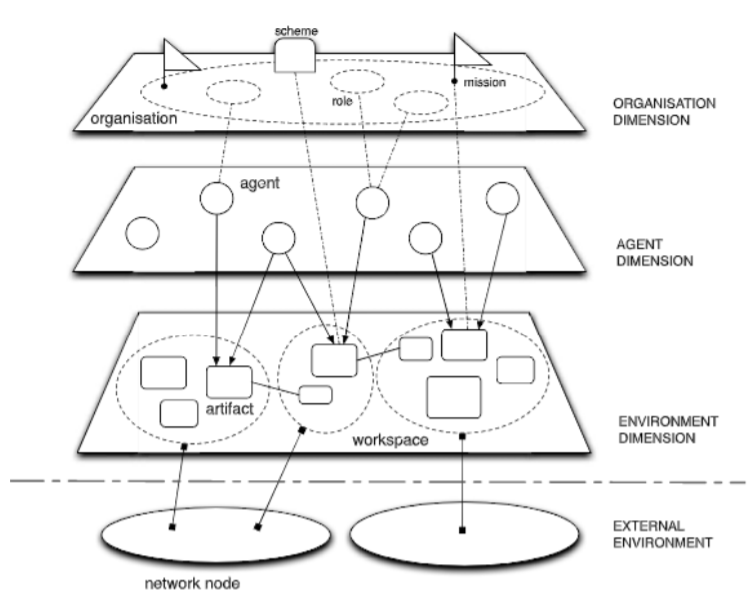
\includegraphics[width=8cm]{images/jacamo_overview.png}
    \caption{Overview of a JaCaMo Multi-Agent System}
    \cite{boissier2013multi}
    \label{fig:jacamo-overview}
\end{figure}

\section{Approach}\label{sec:approach}

Our approach is based on the following three steps:

\subsection{Environment}

Our environment simulates a data center plant. It has several racks, and each rack has several servers. The cells with servers are marked as "gray" and the agents does not move to these cells until the servers are broken. Cells with hardware issues are marked as "red" and cells with software issues are marked as "orange". When an agent tries to solve an issue, it will move to these cells. Free cells are marked as "white" and the agents can move to these cells. In the Figure 3.1, we can see the map that represents the environment.

\begin{figure}[ht]
    \centering
    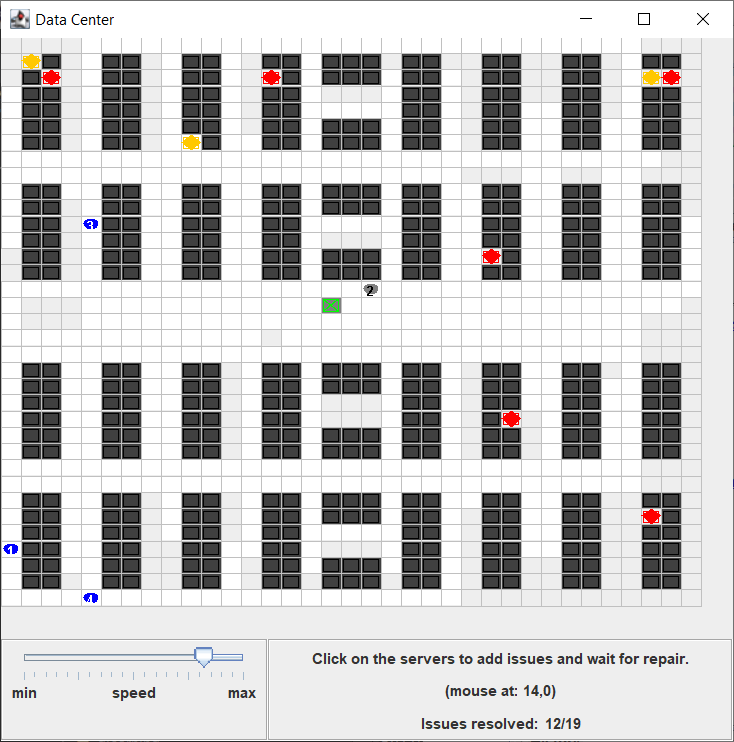
\includegraphics[width=8cm]{images/world.png}
    \caption{Data Center - Environment}
    \label{fig:data-center-env}
\end{figure}

\subsection{Problem}

The problem that our agents are trying to solve is to find all the issues in the data center environment. For that, agents will walk around the environment and try to find issues. When an agent finds an issue, it will try to solve it. If all the issues are solved, the agents still walk around searching for new issues as we can interact with the environment in real time adding new issues.

\subsection{Agents}

Basically, we have two types of agents, the manager and the workers, for the workers, we will have different goals and behaviours.

The \textbf{manager} is responsible for coordinating the workers, it isn't visible in the environment, but it will manage the team scores. We introduced the concept of teams. Currently, each team has only one agent, but we can add more agents for these teams. In the end, the manager will say the team that has the highest score.

The \textbf{technician} agents represent possible roles in a data center such as "facilities technician", "hardware engineer", "network engineer" and "system administrator". They will try to solve the issues in the environment. When they find an issue, they will try to solve it. If they succeed, they will get a score. Software issues only can be solved by the System Admin agent and hardware issues can be solved by the other agents.

We also have the concept of the team. In our experiments, we added one agent per team, but we can add more agents in each team. The manager calculates the score of the teams.

\section{Experiments}\label{sec:experiments}

We developed one scenario to test our Multi-Agent System. This scenario starts with 3 software issues and 19 hardware issues. We also can add more issues by clicking in a server in the world interface, when we add an issue manually, the issue type (hardware or software) will be defined randomly.

Our agents starts walking around the world and try to find and solve the issues.When all issues are solved, the agents still have to walk around the world because new issues can be occurred.

\section{Discussion, Conclusion, and Future Works}\label{sec:conclusions}

In this work, we can conclude that we can build a Multi-Agent System to control autonomous agents in a data center world.

For future work, we want to specify different types of issues handled by each agent and define if agent should return to the command center or not based on the issue type. We also can add more components in the infrastructure such as network devices, air conditioning, and so on.

\bibliographystyle{aaai}
\bibliography{references.bib}

\end{document}